\section{Weighted limits.}\label{section:weight}
The theory of weighted co/limits is a cornerstone of enriched category theory: it can be easily formulated and understood in terms of co/end calculus.

The material presented in this chapter comes from \cite[\textbf{II.7}]{riehl2014categorical}; even the notation is partly unchanged. A more classical reference for the subject is \cite{kelly1982basic,kelly1974review}: we do not make any attempt to recall the fundamental definitions of enriched category theory, heavily relying on these classical references, together with \cite{Bor2}.

It's easy to motivate why co/limits are a fundamental entity of basic category theory. Nevertheless, this notion becomes too strict when one deals with enriched categories; the ``conical'' shape of a classical co/limit is not general enough to encompass the fairly rich variety of shapes in which co/limits in enriched categories arise (the reader has to keep in mind, here, that enriched categories constitute a model for higher category theory; there bare co/limits are ill\hyp{}behaved in several respects, and they must be replaced by their \emph{derived} counterpart); na\"ively speaking, \emph{one} of these shapes gives rise to the notion of a \emph{cone} for a functor $F\colon \cate{J}\to \C$, having as limit the well-known initial/terminal object in a suitable category of diagrams to/from $F$. The theory of weighted co/limits is based on the idea that in its full generality a co/limit takes \emph{two} arguments: the diagram $F$ \emph{of which} we want to compute the co/limit, a presheaf $W \in\widehat{\C}$ \emph{along which} we `weight' the co/limit: conical colimits arise when we choose the terminal presheaf that sends every object of $\C$ on the singleton of $\Sets$.

We cannot touch but the surface of this intricate topic: the interested reader can consult \cite{2catlimits}, a presentation of unmatched lucidity filled with enlightening examples. We choose to follow a relativel more modern approach, for we are interested in translating the fundamentals about weighted co/limits into a \emph{kata} of co/end-fu. %To do this, we follow another really useful and well-written presentation of the theory, \emph{c'est \`a dire} \cite{riehl2014categorical}.\footnote{The reader is warned, now, that the present section results in a rough imitation of this source. Every error is obviously due to the author's misunderstanding.}
\paragraph{\bf Local notation.} Throughout this section, \emph{weight} is a synonym of \emph{presheaf}; we call \emph{ordinary} a category which is enriched over $\Sets$ with its obvious cartesian closed structure.
\subsection[The category of elements of a presheaf.]{A brief prelude: the category of elements of a presheaf.}
\begin{definition}\label{eltsf}
Let $W\colon \C\to \Sets$ be a functor; the \emph{category of elements} $\elts{\C}{W}$ of $W$ is the category having objects the pairs $(c\in\C, u\in Wc)$, and morphisms $(c,u)\to (c',v)$ those $f\in \C(c,c')$ such that $W(f)(u)=v$.
\end{definition}
\begin{notat}
The somewhat exotic notation ``$\elts{\C}{W}$'' for the category of elements of $W$ is inspired by the wondrous paper \cite{Graya}. Other references call it $\int W$ (it is obvious why we can't stick to this more compact notation) or $\text{Elts}(W)$.
\end{notat}
\begin{proposition}
The category $\elts{\C}{W}$ defined in \refbf{eltsf} can be equivalently characterized as each of the following:
\begin{enumerate}[label=$\roman*$)]
\item The category which results from the pullback 
\[
\xymatrix{
  \elts{\C}{W}\ar[r]\ar[d]\ar@{}[dr]|\lrcorner & \Sets_* \ar[d]^U \\
  \C \ar[r]_W & \Sets
}
\]
where $U\colon \Sets_*\to\Sets$ is the forgetful functor which sends a pointed set to its underlying set;
\item The comma category \cite[]{} of the cospan $\{*\}\to \Sets \xot{W} \C$, where $\{*\}\to \Sets$ chooses the terminal object of $\Sets$;
\item The opposite of the comma category $(\yon_{\C}\downarrow \lceil W\rceil)$, where $\lceil W\rceil\colon \{*\}\to [\C, \Sets]$ is the \emph{name} of the functor $W$, \ie the unique functor choosing the presheaf $W\in [\C, \Sets]$:
\begin{center}
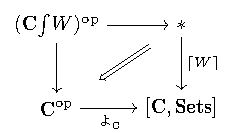
\includegraphics[scale=1]{figures/fig5}
\end{center}
\end{enumerate}
\end{proposition}
\begin{proof}
The proof that these categories are all canonically isomorphic to $\elts{\C}{W}$ is an exercise in Yoneda lemma and universal properties that we leave to the reader.
\end{proof}
\begin{remark}
There is a fourth characterization for the category of elements of a presheaf that couches it as a particular weighted colimit which, using the formalism exposed in this section, can be written as a coend. Example \refbf{elts-as-coend} below is a guided exercise in proving and clarifying this statement.
\end{remark}
\begin{proposition}\label{fibelem}
The category of elements $\elts{\C}{W}$ of a functor $W\colon \C\to \Sets$ comes equipped with a canonical Grothendieck fibration \cite[\adef\refbf{}]{Bor2} to the domain of $W$, which we denote $\Sigma\colon \elts{\C}{W}\to \C$, defined forgetting the distinguished element $u\in Wc$. 
\end{proposition}
\begin{proof}
We only have to prove that $\Sigma \colon \elts{\C}{W}\to \C$ is an isofibration; given an isomorphism $\phi\colon x\to c=\Sigma(c,u)$, we can define $v\in Wx$ to be $W(\phi^{-1})(u)$.
\end{proof}
\begin{notat}\label{cosmo}
All along the present section, we assume that $\V$ denotes a \emph{B\'enabou cosmos} \cite[???]{cosmo-ref}, \ie a symmetric monoidal closed, complete and cocomplete category which is the ``base'' for our enriched category theory.
\end{notat}
\begin{remark}
Let $F\colon \cate{J}\to\C$ be a functor between small ordinary categories. The \emph{limit} $\varprojlim F$ of $F$ can be characterized as the representing object of a suitable presheaf: indeed, we have the natural isomorphism
\[
\C(c, \varprojlim F)\cong \Set^\cate{J}(*, \C(c,F(\firstblank)))
\]
where $*$ is a shorthand to denote the terminal functor $\cate{C}\to \Sets \colon c\mapsto *$ sending every object to the terminal set, and $\C(a,F(\firstblank))$ is the functor $\cate{J}\to \Sets$ sending $j$ to $\A(c, Fj)$.

Dually, the colimit $\varinjlim F$ of $F\colon \cate{J}\to \C$ can be characterized, in the same notation, as the representing object in the natural isomorphism
\[
\cate{J}(\varinjlim F,c)\cong \Set^\cate{J}(*, \cate{J}(F(\firstblank),c)).
\]
\end{remark}
$\Set^\cate{J}(*, \C(F,c))$ is a set of natural transformations and $c\mapsto \Set^\cate{J}(*, \A(F,c))$ is a functor: the leading idea behind the definition of weighted co/limit is to generalize this construction to admit shapes other than the terminal presheaf for the domain functor.  We can package this intuition in the following definition:
\begin{definition}[Weighted limit and colimit]\label{weightdef}
Given functors $F\colon \cate{J}\to  \C$ and $W\colon \cate{J}\to \Set$, we define the \emph{weighted limit} of $F$ by $W$ as a representative for the functor sending $c\in \C$ to $\Set^\cate{J}(W, \C(c, F(\firstblank)))$, in other words the weighted limit of $F$ by $W$ is an object $\wlim{W}F\in \C$ such that
\[\textstyle  \C\big(c,\wlim{W}F\big)\cong \Set^\cate{J}(W, \C(c,F(\firstblank)))\]
naturally in $c\in \C$. Dually we define the \emph{colimit} of $F\colon \cate{J}\to \C$ weighted by $W\colon\cate{J}^\opp\to\Set$ to be an object $\varinjlim^WF\in \C$ such that
\[\textstyle  \C\big(\wcolim{W}F, c\big)\cong \Set^{\cate{J}^\opp}(W, \C(F(\firstblank),c)).\]
\end{definition}
\begin{example}\label{frecc}
Let $f\colon \Delta^1\to\C$ the functor choosing an arrow $f\colon x\to y$ in $\C$, and $W\colon \Delta^1\to \Set$ the functor sending $\{0<1\}$ to the single arrow $\{0,1\}\to \{0\}$; then a natural transformation $W\Rightarrow \C(c,f)$ consists of arrows $W0\to \C(c,x), W1\to \C(c',y)$, namely on the choice of two arrows $h,k\colon c\to x$ such that $fh=fk$: the universal property for $\varprojlim^Wf$ implies that this is the \emph{kernel pair} of the arrow $f$, namely that $h,k$ fill in the pullback
\[
\xymatrix@R=8mm@C=8mm{
c\ar@/^1pc/[drr]^h\ar@/_1pc/[ddr]_k\ar@{.>}[dr] & \\
& \varprojlim^Wf\ar[r]\ar[d] \ar@{}[dr]|\lrcorner & x \ar[d]^f \\
& x\ar[r]_f & y
}
\]
\end{example}
The next result is the awaited characterization of weighted co/limits as co/ends:
\begin{proposition}[Weighted co/limits as co/ends]\label{wlimcoends}
When the end below and the $\Sets$-cotensor $(X, a)\mapsto a^X$ exist, we can express the weighted limit $\wlim{W}F$ for $F \colon \cate{J}\to \C$ as an end using the chain of isomorphisms
\begin{align*}
\Set^\cate{J}(W,\C(c,F))
& \cong \int_{j\in\cate{J}}\Set(Wc, \C(c, Fj))\\
& \cong \int_{j\in\cate{J}}\C\big(c, Fj^{Wj}\big)\\
& \cong \C\Big(c,\int_{j\in\cate{J}} Fj^{Wj}\Big)
\end{align*}
and the uniqueness for a representing object. Indeed, the above string of natural isomorphisms implies that there is a canonical isomorphism
\[
\wlim{W}F\cong \int_{j\in\cate{J}} Fj^{Wj}
\]
\end{proposition}
\begin{example}
Consider the particular case of two parallel functors $W,F\colon \C\to\Sets$; then we can easily see that $\wlim{W}F$ coincides with the set of natural transformations $W\Rightarrow F$, since the cotensor $Fc^{Wc}$ is precisely the set $\Sets(Wc, Fc)$.
\end{example}
\begin{example}
The ninja Yoneda lemma \refbf{ninjayo}, rewritten in this notation, says that $\wlim{\C(c,\firstblank)}F\cong Fc$ (or, in case $F$ is contravariant, $\wlim{\C(\firstblank,c)}F\cong Fc$). This can be memorized as ``representably\hyp{}weighted co/limits are evaluation'' (see Remark \refbf{dirac} on the `Dirac delta') and suggests that \emph{Kan extensions} can be expressed as suitable weighted co/limits, and more precisely that they can be characterized as those weighted co/limits where the weight is a representable functor:
\[
\Ran_KF(\firstblank) \cong \int_{c\in\C} Fc^{\D(\firstblank, Kc)}\cong \wlim{\D(\firstblank, K\secondblank)}F.
\]
\end{example}
The following Remark and Proposition constitute a central observation.
\begin{remark}[\righteyes, The Grothendieck construction trivializes weights]
Definition \refbf{weightdef} can be extended in the case $F\colon \C\to\A$ is a $\V$-enriched functor between $\V$-categories, and $W\colon \C\to\V$ is a $\V$-co/presheaf; this is the setting where the notion of a weighted co/limit acquires a supremacy over the ``classical'' one (where the weight is the terminal presheaf). When $\V=\Sets$, indeed, the \emph{Grothendieck construction} sending a (co)presheaf into its category of elements turns out to trivialize almost completely the theory of $\Sets$-weighted limits: as the following discussion shows, in such a situation every weighted limit can be expressed as a classical (we call them \emph{conical}, due to the shape of the weight) limit.
\end{remark}
\begin{proposition}[$\Sets$-weighted limits are limits]\label{elementi}
As shown in Prop\@. \refbf{fibelem}, the category $\elts{\C}{W}$ comes equipped with a fibration $\Sigma\colon \elts{\C}{W}\to\C$, such that for any functor $F\colon \C\to \A$ one has 
\[\wlim{W}F\cong \varprojlim_{(c,x)\in \elts{\C}{W}} F\circ \Sigma.\]
\end{proposition}
\begin{proof}
The proof goes by inspection, using the characterization of the end $\int_{c\in \C}Fc^{Wc} $ as an equalizer (see Proposition \refbf{endsareeq}), and the characterization of $\Sets$-cotensors as iterated products, showing that 
\begin{align*}
\int_{c\in \C}Fc^{Wc} &\cong {\rm eq}\Big(  \prod_{c\in \C}Fc^{Wc}\rightrightarrows \prod_{c\to c'}Fc'^{Wc}\Big)\\
&\cong {\rm eq}\Big( \prod_{c\in\C}\prod_{x\in Wc} Fc\rightrightarrows \prod_{c\to c'}\prod_{x\in Wc}Fc' \Big)\\
(\star) &\cong {\rm eq}\Big( \prod_{(c,x)\in \elts{\C}{W}} Fc\rightrightarrows \prod_{(c,x)\to (c',x')\in \elts{\C}{W}} Fc' \Big)\\
&\cong \varprojlim_{(c,x)\in\elts{\C}{W}} F\circ \Sigma 
\end{align*}
(equation $(\star)$ is motivated by the fact that every arrow $\phi \colon \Sigma(c,x)\to c'$ has a unique lift $(c,x)\to (c', x')$ since $W(\phi)(x) = x'm$).
\end{proof}
\begin{remark}
When we consider Kan extensions as weighted co/limits, this result agrees with the classical theory: if the weight has the form $W=\D(d,K-)$ for an object $d\in\D$, and a functor $K\colon \C\to\D$, then the category of elements $\elts{\C}{W}$ is precisely the \emph{comma category} $(d\downarrow K)$: the right Kan extension of $F$ along $K$ can be computed as the conical limit of the functor $FU$, where $U\colon (d\downarrow K)\to \C$ is the obvious forgetful functor.
\end{remark}
Obviously, when \emph{every} weighted limit exists in $\A$, we can prove that the correspondence $(W,F) \mapsto\wlim{W}F$ is a bifunctor:
\[
\wlim{(\firstblank)}\,(=)\colon \big(\Sets^\C \big)^\opp\times \A^\C\longrightarrow \A.
\] A number of useful corollaries of this fact:
\begin{itemize}
\item The unique, terminal natural transformation $W\to *$ induces a \emph{comparison arrow} between the weighted limit of any $F\colon\C\to\A$ and the classical (conical) limit: $\varprojlim F\to \wlim{W}F$. For example, the classical limit of the functor $f\colon \Delta[1]\to \A$ described in Example \refbf{frecc} consists of the object $a = \text{src}(f)$; hence the comparison arrow consists of the unique factorization of two copies of $\id_a$ along the kernel pair of $f$.
\item The functor $\wlim{(\firstblank)}F$ is continuous, namely we can prove the suggestive isomorphism
\[\textstyle\label{wlimcocont} 
\wlim{\big(\varinjlim_J W_j\big)}F\cong \varprojlim_J \big(\wlim{W_j}F\big),
\]
valid for any small diagram of weights $\cate{J}\to [\C, \Sets]\colon j\mapsto W_j$.
\end{itemize}
\begin{example}\label{ends-are-weighted}
Ends can be computed as weighted limits: given $H\colon \C^\opp\times\C\to\D$ we can take the hom functor $\C(\firstblank,\secondblank)\colon \C^\opp\times\C\to\Sets$ as a weight, and if the weighted limit exists, we have the chain of isomorphisms
\[
\wlim{\C(\firstblank,\secondblank)}H\cong \int_{(c,c')\in \C^\opp\times\C } H(c,c')^{\C(c,c')}\cong 
\int_c \Big( \int_{c'}H(c,c')^{\C(c,c')}\Big)\stackrel{\refbf{ninjayo}}{\cong}\int_c H(c,c).
\]
\end{example}
\begin{remark}
This characterization will turn out to be useful during our discussion of \emph{simplicially coherent} co/ends. See \refbf{cohcoend}.
\end{remark}
\begin{remark}
Weighted \emph{colimits} are discussed in Exercise \refbf{ex4:wcolims} and stem from a straightforward dualization process; we refer freely to both concepts from now on.
\end{remark}
\begin{remark}
Aside from showing that ``weighted limits are the true enriched-categorical limits'', the above examples and the last characterization of ends as weighted limits are fundamental steps towards a sensible definition of \emph{enriched} ends: given a B\'enabou cosmos $\V$ (see Notation \refbf{cosmo}) and a $\V$-functor $H\colon \C^\opp\times\C\to\V$, we \emph{define} $\int_c H(c,c)$ to be the limit of $H$ weighted by $\C(\firstblank,=)\colon \C^\opp\boxtimes\C\to\V$ (see Definition \refbf{cosmuclosed} for the notation $\C\boxtimes \D$).
\end{remark}
\begin{remark}\label{homcommuteswei}
Let $F\colon \C \to \A, W\colon \C \to \V, U\colon \C^\opp\to \V$ be $\V$-functors and let $\A$ be $\V$-tensored. There are canonical isomorphisms
\begin{gather}
\A(\wcolim{W}F,x)\cong \wlim{W}\A(F,x)\\
\A(y, \wlim{U}F)\cong \wlim{W}\A(y, F).
\end{gather}
This can be recorded in the motto ``the hom functor commutes with weighted limits'' (prove it as an exercise).
\end{remark}
\begin{example}[The cone construction as a weighted colimit]\label{cone-is-a-colim}
Let $K$ be a ring, and $\V = \cate{Ch}(K)$ the category of chain complexes of $K$-modules. Considering $\V$ as a $\V$-category in the obvious way, we aim to prove that the \emph{mapping cone} $\text{C}(f) = X_*[1]\oplus Y_*$ of a chain map $f\colon X_*\to Y_*$ \cite[\textbf{1.5.1}]{Weibel1994} in $\V$ can be characterized as the weighted colimit $\wcolim{W}f$, where $f\colon \Delta[1]\to \V$ is the arrow $f$, and $W\colon \Delta[1]^\opp\to \V$ is the functor which chooses the map $S^1(K)_*\to D^2(K)_*$, where $S^n(K)_* = K[n]_*$ is the chain complex with the only term $K$ concentrated in degree $-n$, and $D^n(K)_*$ is the complex
\begin{equation*}
\xymatrix{
\cdots \ar[r]& 0 \ar[r] & K \ar@{=}[r] & K \ar[r] & 0 \ar[r] & \cdots,
}
\end{equation*}
where the first nonzero term is in degree $-n$. There is an obvious inclusion $S^n_* \hookrightarrow D^{n+1}_*$:
\begin{equation*}
\xymatrix{
\cdots \ar[r]& 0 \ar[r] & 0 \ar[d] \ar[r] & K \ar[r] \ar@{=}[d] & 0 \ar[r] & \cdots \\
\cdots \ar[r]& 0 \ar[r] & K \ar@{=}[r] & K \ar[r] & 0 \ar[r] & \cdots.
}
\end{equation*}
We now aim to prove that 
\begin{equation} \label{eq:cap2_cone_coend}
\text{C}(f) \cong \int^{i \in \Delta^1} W(i) \otimes f(i).
\end{equation}
In view of (the dual of) Exercise \textbf{1}.\refbf{ispull}, it is enough to show that there is a pushout square
\begin{equation*}
\xymatrix{
W(1) \otimes f(0)\ar@{}[dr]|\ulcorner \ar[r] \ar[d] & W(1) \otimes f(1) \ar@{.>}[d]\\
W(0) \otimes f(0) \ar@{.>}[r]& \text{C}(f)
}
\end{equation*}
This is a rather simple exercise in universality, given the maps
\[
\xymatrix@C=2cm{
  B \ar[r]^{\left(\begin{smallmatrix} 0\\1 \end{smallmatrix}\right)} & \text{C}(f) & \ar[l]_{\left(\begin{smallmatrix} 0 & 1 \\ f & 0 \end{smallmatrix}\right)} A\oplus A[1].
}
\]
\end{example}
\begin{example}[The category of elements of a presheaf]\label{elts-as-coend}
The scope of this example is to prove that the category of elements of a functor $F\colon \C\to \Sets$ introduced in Def\@. \refbf{eltsf} can be characterized as a $\Cat$-weighted colimit: it is, in particular, the category isomorphic to the colimit
\[
{\textstyle \elts{\C}{W}}\cong \int^{c\in\C} c/\C \times Wc
\]
where $Wc$ is the set, regarded as a discrete category; it is, in other words, isomorphic to the weighted colimit $\wcolim{J}{W}$, where $J\colon \C^\opp\to \Cat$ is the functor $c\mapsto c/\C$ (the ``coslice'' category of arrows $c\to x$).

To prove this statement, we verify that $\elts{\C}{W}$ has the universal property of the coequalizer of the pair
\[
\xymatrix{
	\displaystyle \coprod_{f\colon a\to b} b/\C \times Wa \ar@<4pt>[r]^\alpha \ar@<-4pt>[r]_\beta & \displaystyle \coprod_{c\in\C} c/\C \times Wc
}
\]
where $\alpha$ has components $\alpha_f \colon b/\C \times Wa \xto{1\times Ff} b/\C \times Wb$ sending $\left(\var{b}{x}, u\right)\mapsto \left( \var{b}{x}, F(f)u \right)$ and $\beta$ has components $\beta_f \colon b/\C \times Wa\xto{f^*\times Wa} a/\C \times Wa$ sending  $\left(\var{b}{x}, u\right)\mapsto \left( \left[\begin{smallmatrix} a &\xto{f} & b \\ &&\downarrow \\ && x \end{smallmatrix}\right], u \right)$.

It's rather easy to define a functor
\[
\theta\colon \coprod_{a\in\C} a/\C\times Wa \longrightarrow \textstyle \elts{\C}{W}
\]
having components $\theta_a \colon a/\C\times Wa \to \elts{\C}{W}$ sending $\left( \var[\!\! f]{a}{b}, u\in Fa\right)\mapsto \left( b , F(f)(u)\in Fb\right)$, which coequalizes $\alpha$ and $\beta$. This functor $\theta$ has the universal property of the coequalizer: given any other $\zeta\colon \coprod_{a\in\C} a/\C\times Wa \to \cate{K}$ we can define a functor $\overline{\zeta}\colon \elts{\C}{W}\to \cate{K}$ such that
\[ \overline{\zeta}(a, u\in Fa) = \zeta(\id_a, u). \]
Now notice that every map $\zeta'$ that coequalizes $(\alpha,\beta)$ has the property that
\[ 
\zeta'\left( \var[g]{b}{x}, F(f)u \right) = \zeta'\left( \left[\begin{smallmatrix} a &\xto{f} & b \\ &&\downarrow \\ && x \end{smallmatrix}\right] , u \right)
\]
It is now a routine verification to see that $\overline{\zeta}\circ\theta_a = \zeta_a$, and every other functor with this property must coincide with our $\overline{\zeta}$. This concludes the proof.
\end{example}
\begin{remark}\label{its.another.nerve}
The careful reader may have noticed that all the above discussion gives a fifth presentation for the category of elements $\elts{\C}{W}$, as the image of $W$ under the Kan extension $\Lan_\yon J$: in the language of \S\refbf{section:nr}, $J\colon \C^\opp\to \Cat$ is the \textsc{nr}-context of the paradigm
\[
\xymatrix{
\elts{\C}{\firstblank} \colon [\C, \Sets]  \ar@<4pt>[rr]&& \ar@<4pt>[ll] \Cat\colon N_J
}
\]
where $N_J\colon \Cat \to  [\C, \Sets] $ is the ``nerve'' functor sending $\A$ to $c\mapsto \Cat(c/\C, \A)$.
\end{remark}
\begin{remark}
An alternative approach to characterize $\elts{\C}{W}$ is the following: the category $\elts{\C}{W}$ is precisely the lax limit of $W$ regarded as a $\Cat$-valued presheaf \cite[\S\textbf{4}]{2catlimits}, \cite{Graya,Street19}.
\end{remark}
A fundamental step to write the theory of weighted limits relies upon the above-mentioned isomorphism
\[
\A\big(m,\wlim{W}F\big) \cong \V^{\C}(W, \A(m,F(\firstblank)))
\]
valid in a $\V$-category $\A$ naturally in any object $m\in\A$; this isomorphism has to be interpreted in the base-cosmos $\V$, and this means that we have to find a way to interpret the category $\V^\C$ as an object $[\cate C,{\V}]$ of $\V$: to do this, we must endow $\V\text{\firstblank}\Cat$ with a closed symmetric monoidal structure, such that
\[\label{closurenrich}
\V\text{-}\Fun(\C\boxtimes \cate{E}, \D) \cong 
\V\text{-}\Fun(\cate{E}, [\C,\D]).
\]
\begin{definition}\label{cosmuclosed}
Given two $\V$-categories $\C, \D$ we define the $\V$-category $\C\boxtimes\D$ having
\begin{itemize}
\item as objects the set $\C\times\D$, and 
\item as $\V$-object of arrows $(c,d)\to (c',d')$ the object
\[
\C(c,c')\otimes \D(d,d')\in\V.
\]
\end{itemize}
The free $\V$-category $\cate{I}$ associated to the terminal category is the unit object for this monoidal structure.
\end{definition}
\begin{proposition}
$(\VCat,\boxtimes)$ is a closed monoidal structure, with internal hom denoted $[\firstblank,\secondblank]\colon \VCat^\opp\times \VCat \to \VCat$.
\end{proposition} 
\begin{proof}
Given $\C,\D\in \VCat$ we define a $\V$-category whose objects are $\V$-functors $F,G\colon \C\to\D$ and where (`abstracting' Theorem \refbf{naturalu} to the enriched setting) the $\V$-object of natural transformations $F\Rightarrow G$ is defined via the end
\[
[\C,\D](F,G) := \int_{c\in\C} \D(Fc,Gc).
\]
Recall that in the unenriched case, the end was better understood as the equalizer of a pair of arrows:
\[
\int_{c\in\C}\D(Fc,Gc)\cong {\rm eq}\Big( \prod_{c\in \C}\D(Fc,Gc)\rightrightarrows \prod_{c,c'}\prod_{c\to c'}\D(Fc,Gc') \Big)
\]
In the enriched case, we can consider the same symbol, and re-interpret the product $\prod_{\C(c,c')}$ as a suitable \emph{power} in $\V$:
\[
\int_{c\in\C}\D(Fc,Gc)\cong {\rm eq}\Big( \prod_{c\in \C}\D(Fc,Gc)\rightrightarrows \prod_{c,c'} \D(Fc,Gc')^{\C(c,c')}\Big)
\]
(see also \cite[\S \textbf{2.3}]{Gray1980}, \cite{dubuc1970kan} for a more detailed discussion about co/ends in enriched setting.)

It remains to prove, now, that the isomorphism (\refbf{closurenrich}) holds: this is rather easy, since in the above notations, any functor $F\colon \C\boxtimes \cate{E} \to \D$ defines a unique functor $\hat F\colon \cate E \to [\C,\D]$.\footnote{Notice that for any two objects $e,e'\in\cate{E}$, the collection of arrows $\hom(e,e') \to \hom(F(c,e) , F(c,e')]$ is a wedge in $c\in\C$.}
\end{proof}
The given definition for the enriched end allows us to state an elegant form of the $\V$-enriched Yoneda lemma:
\begin{remark}[$\V$-Yoneda lemma]
Let $\D$ be a small $\V$-category, $d\in\D$ an object, and $F\colon \D\to\V$ a $\V$-functor. Then the canonical map
\[
Fd\longrightarrow [\D,\V](\D(d,\firstblank),F)
\]
induced by the universal property of the involved end\footnote{Notice that this is an alternative point of view on the proof of the ninja Yoneda lemma \refbf{ninjayo}; this arrow is induced by a wedge $\{Fd\to \V(\D(d,a), Fa)\}_{a\in\C}$, whose members are the mates of the various $\D(d,a)\to \V(Fd,Fa)$ giving the action of $F$ on arrows.} is a $\V$-isomorphism.
\end{remark}
\paragraph{\bf Homotopy co/limits as weighted co/limits.}
We can express the Bousfield\hyp{}Kan construction for the homotopy co/limit functor using co/end calculus (see \refbf{coends-in-model} for a crash course on what's an homotopy co/limit). We condense Bousfield\hyp{}Kan construction in the following series of examples.
\begin{theorem}[The Bousfield-Kan formula for homotopy co/limits]
Let $F \colon \cate{J}\to \M$ be a diagram in a model category $(\M, \wk,\cof,\fib)$ which is tensored and cotensored over the category $\sSet$ of simplicial sets by functors $\pitchfork \colon \sSet^\opp\times \M \to \M$ and $\cdot \colon \sSet \times \M \to \M$. Then the homotopy limit $\holim F$ of $F$ can be computed as the end
\[
\int_j N(J/j)\pitchfork F(j),
\]
and the homotopy colimit $\hocolim F$ of $F$ can be computed as the coend
\[
\int^j N(j/J) \cdot F(j).
\]
\end{theorem}
\begin{remark}
These two universal objects are weighted co/limits in an evident way: it is possible to rewrite $\holim F\cong \wlim{N(J/\firstblank)}F$ and $\hocolim F\cong \wcolim{N(\firstblank/J)}F$.

The idea behind this characterization is that the co/limit functor results as the weighted colimit over the terminal weight or in \cite{}'s notation $\{*,F\}$ and $*\otimes F$. When we want to pass to the homotopy invariant version of the $\wcolim{(\firstblank)}{(\secondblank)}$ bifunctor we can choose to `replace' the diagram part $F$ or the weight $W$ with a more homotopically\hyp{}well\hyp{}behaved diagrams $\hat F$ or $\tilde W$. Bousfield\hyp{}Kan formula arises precisely when we derive the weight: $N(j/J)$ and $N(J/j)$ are contractible categories, and they are linked to $N(*)$ by an homotopy equivalence induced by the terminal functor.

Then, the categories $N(J/\firstblank),N(\firstblank/J)$ must be thought as proper \emph{replacements} for the co/limit functor that correct its failure to preserve weak equivalences (see \cite{strom} for an extremely hands-on account of the theory of homotopy co/limits).
\end{remark}
\begin{example}
The \emph{mapping cylinder} of $f \colon A \to B$ is the topological space obtained from $\big(A\times[0,1]\big) \coprod B$ from the smallest quotient that identifies $(f(a), (a, 0))$ for all $a \in A$ (compare this example with Example \refbf{cone-is-a-colim} and Exercise \refbf{ex:cone-again} below).
\end{example}
\begin{exerciseset}
\begin{exercisepoints}
\item Prove Equation (\refbf{wlimcocont}) using the characterization of $\wlim{W}F\cong \int_c Fc^{Wc}$, plus its universal property.
\item What is the category of elements of the hom functor? Compare with Definition \refbf{twisted}.
\item \label{ex4:wcolims} Every definition we gave until now can be dualized to obtain a theory of weighted \emph{co}limits: fill in the details.
\begin{enumerate}[label=$\roman*$)]
	\item (weighted colimits as coends) If $\A$ is cocomplete, we can express the weighted colimit $\wcolim{W}F$ as a coend: more precisely
	\[
	\wcolim{W}F\cong \int^{c\in\C} Wc\cdot Fc
	\] 
	where we used, like everywhere else, the $\Sets$-tensoring of $\A$.
	\item (left Kan extensions as weighted colimits) Let $F\colon \C\to \A$ and $K\colon \C\to \D$ be functors; then 
	\[
	\Lan_KF(\firstblank)\cong \int^{c\in\C} \D(Kc,\firstblank)\cdot Fc\cong \wcolim{\D(K\secondblank,\firstblank)}F
	\]
	\item (coends as $\hom$-weighted colimits) The coend of $H\colon \C^\opp\times\C\to \D$ can be written as  $\wcolim{\C(\firstblank,\secondblank)}H$.
	\item If the weight $W$ is $\Sets$-valued, the colimit of $F$ weighted by $W$ can be written as a conical colimit over $\elts{\C^\opp}{W}$: 
	\[
	 \wcolim{W}F\cong \varinjlim_{(c,x)\in \elts{\C^\opp}{W}}F\Sigma
	\]
	\item (functoriality) If the $W$-colimit of $F\colon\C\to\A$ always exists, then the correspondence $(W,F)\mapsto \wcolim{W}F$ is a functor, cocontinuous in its first variable:
	\begin{gather}
	\wcolim{(\firstblank)}(=)\colon \Sets^{\C^\opp} \times \A^\C\longrightarrow \A, \notag \\
	\textstyle 
	\wcolim{\big(\varinjlim_J W_j\big)}F\cong \varinjlim_J \big(\wcolim{W_j}F\big)
	\end{gather}
	\item (comparison) There is a canonical natural transformation $W\to *$, inducing a canonical \emph{comparison arrow} from the $W$-colimit of any $F\colon \C\to \A$ to the conical colimit.
\end{enumerate}
\item \label{ex:cone-again} Let $w\colon S^0 \hookrightarrow D^1$ be the canonical inclusion of $\{0,1\}$ into $[0,1]\subset \mathbb{R}$, with the usual topology; prove that the mapping cone of a continuous map $f\colon X\to Y$ is precisely the weighted colimit $\wcolim{w}f$.
\item Fill in the details of the above proof; for those who need a hint, show that $\cate E(e, e')\to \D(F(x,e), F(x, e'))$ is a wedge in $x\in \C$.
\item Show that there are canonical isomorphisms $\wlim{W}FJ\cong \wlim{\Lan_JW}F$, and dually $\wcolim{WJ}F\cong \wcolim{W}\Lan_JF$.
\end{exercisepoints}
\end{exerciseset}
